
%% bare_conf.tex
%% V1.3
%% 2007/01/11
%% by Michael Shell
%% See:
%% http://www.michaelshell.org/
%% for current contact information.
%%
%% This is a skeleton file demonstrating the use of IEEEtran.cls
%% (requires IEEEtran.cls version 1.7 or later) with an IEEE conference paper.
%%
%% Support sites:
%% http://www.michaelshell.org/tex/ieeetran/
%% http://www.ctan.org/tex-archive/macros/latex/contrib/IEEEtran/
%% and
%% http://www.ieee.org/

%%*************************************************************************
%% Legal Notice:
%% This code is offered as-is without any warranty either expressed or
%% implied; without even the implied warranty of MERCHANTABILITY or
%% FITNESS FOR A PARTICULAR PURPOSE! 
%% User assumes all risk.
%% In no event shall IEEE or any contributor to this code be liable for
%% any damages or losses, including, but not limited to, incidental,
%% consequential, or any other damages, resulting from the use or misuse
%% of any information contained here.
%%
%% All comments are the opinions of their respective authors and are not
%% necessarily endorsed by the IEEE.
%%
%% This work is distributed under the LaTeX Project Public License (LPPL)
%% ( http://www.latex-project.org/ ) version 1.3, and may be freely used,
%% distributed and modified. A copy of the LPPL, version 1.3, is included
%% in the base LaTeX documentation of all distributions of LaTeX released
%% 2003/12/01 or later.
%% Retain all contribution notices and credits.
%% ** Modified files should be clearly indicated as such, including  **
%% ** renaming them and changing author support contact information. **
%%
%% File list of work: IEEEtran.cls, IEEEtran_HOWTO.pdf, bare_adv.tex,
%%                    bare_conf.tex, bare_jrnl.tex, bare_jrnl_compsoc.tex
%%*************************************************************************

% *** Authors should verify (and, if needed, correct) their LaTeX system  ***
% *** with the testflow diagnostic prior to trusting their LaTeX platform ***
% *** with production work. IEEE's font choices can trigger bugs that do  ***
% *** not appear when using other class files.                            ***
% The testflow support page is at:
% http://www.michaelshell.org/tex/testflow/



% Note that the a4paper option is mainly intended so that authors in
% countries using A4 can easily print to A4 and see how their papers will
% look in print - the typesetting of the document will not typically be
% affected with changes in paper size (but the bottom and side margins will).
% Use the testflow package mentioned above to verify correct handling of
% both paper sizes by the user's LaTeX system.
%
% Also note that the "draftcls" or "draftclsnofoot", not "draft", option
% should be used if it is desired that the figures are to be displayed in
% draft mode.
%
\documentclass[10pt, a4paper, conference, compsocconf]{IEEEtran}
% Add the compsocconf option for Computer Society conferences.
%
% If IEEEtran.cls has not been installed into the LaTeX system files,
% manually specify the path to it like:
% \documentclass[conference]{../sty/IEEEtran}





% Some very useful LaTeX packages include:
% (uncomment the ones you want to load)


% *** MISC UTILITY PACKAGES ***
%
%\usepackage{ifpdf}
% Heiko Oberdiek's ifpdf.sty is very useful if you need conditional
% compilation based on whether the output is pdf or dvi.
% usage:
% \ifpdf
%   % pdf code
% \else
%   % dvi code
% \fi
% The latest version of ifpdf.sty can be obtained from:
% http://www.ctan.org/tex-archive/macros/latex/contrib/oberdiek/
% Also, note that IEEEtran.cls V1.7 and later provides a builtin
% \ifCLASSINFOpdf conditional that works the same way.
% When switching from latex to pdflatex and vice-versa, the compiler may
% have to be run twice to clear warning/error messages.






% *** CITATION PACKAGES ***
%
%\usepackage{cite}
% cite.sty was written by Donald Arseneau
% V1.6 and later of IEEEtran pre-defines the format of the cite.sty package
% \cite{} output to follow that of IEEE. Loading the cite package will
% result in citation numbers being automatically sorted and properly
% "compressed/ranged". e.g., [1], [9], [2], [7], [5], [6] without using
% cite.sty will become [1], [2], [5]--[7], [9] using cite.sty. cite.sty's
% \cite will automatically add leading space, if needed. Use cite.sty's
% noadjust option (cite.sty V3.8 and later) if you want to turn this off.
% cite.sty is already installed on most LaTeX systems. Be sure and use
% version 4.0 (2003-05-27) and later if using hyperref.sty. cite.sty does
% not currently provide for hyperlinked citations.
% The latest version can be obtained at:
% http://www.ctan.org/tex-archive/macros/latex/contrib/cite/
% The documentation is contained in the cite.sty file itself.






% *** GRAPHICS RELATED PACKAGES ***
%
\ifCLASSINFOpdf
  \usepackage[pdftex]{graphicx}
  % declare the path(s) where your graphic files are
  % \graphicspath{{../pdf/}{../jpeg/}}
  % and their extensions so you won't have to specify these with
  % every instance of \includegraphics
  % \DeclareGraphicsExtensions{.pdf,.jpeg,.png}
\else
  % or other class option (dvipsone, dvipdf, if not using dvips). graphicx
  % will default to the driver specified in the system graphics.cfg if no
  % driver is specified.
  \usepackage[dvips]{graphicx}
  % declare the path(s) where your graphic files are
  % \graphicspath{{../eps/}}
  % and their extensions so you won't have to specify these with
  % every instance of \includegraphics
  % \DeclareGraphicsExtensions{.eps}
\fi
% graphicx was written by David Carlisle and Sebastian Rahtz. It is
% required if you want graphics, photos, etc. graphicx.sty is already
% installed on most LaTeX systems. The latest version and documentation can
% be obtained at: 
% http://www.ctan.org/tex-archive/macros/latex/required/graphics/
% Another good source of documentation is "Using Imported Graphics in
% LaTeX2e" by Keith Reckdahl which can be found as epslatex.ps or
% epslatex.pdf at: http://www.ctan.org/tex-archive/info/
%
% latex, and pdflatex in dvi mode, support graphics in encapsulated
% postscript (.eps) format. pdflatex in pdf mode supports graphics
% in .pdf, .jpeg, .png and .mps (metapost) formats. Users should ensure
% that all non-photo figures use a vector format (.eps, .pdf, .mps) and
% not a bitmapped formats (.jpeg, .png). IEEE frowns on bitmapped formats
% which can result in "jaggedy"/blurry rendering of lines and letters as
% well as large increases in file sizes.
%
% You can find documentation about the pdfTeX application at:
% http://www.tug.org/applications/pdftex





% *** MATH PACKAGES ***
%
%\usepackage[cmex10]{amsmath}
% A popular package from the American Mathematical Society that provides
% many useful and powerful commands for dealing with mathematics. If using
% it, be sure to load this package with the cmex10 option to ensure that
% only type 1 fonts will utilized at all point sizes. Without this option,
% it is possible that some math symbols, particularly those within
% footnotes, will be rendered in bitmap form which will result in a
% document that can not be IEEE Xplore compliant!
%
% Also, note that the amsmath package sets \interdisplaylinepenalty to 10000
% thus preventing page breaks from occurring within multiline equations. Use:
%\interdisplaylinepenalty=2500
% after loading amsmath to restore such page breaks as IEEEtran.cls normally
% does. amsmath.sty is already installed on most LaTeX systems. The latest
% version and documentation can be obtained at:
% http://www.ctan.org/tex-archive/macros/latex/required/amslatex/math/





% *** SPECIALIZED LIST PACKAGES ***
%
%\usepackage{algorithmic}
% algorithmic.sty was written by Peter Williams and Rogerio Brito.
% This package provides an algorithmic environment fo describing algorithms.
% You can use the algorithmic environment in-text or within a figure
% environment to provide for a floating algorithm. Do NOT use the algorithm
% floating environment provided by algorithm.sty (by the same authors) or
% algorithm2e.sty (by Christophe Fiorio) as IEEE does not use dedicated
% algorithm float types and packages that provide these will not provide
% correct IEEE style captions. The latest version and documentation of
% algorithmic.sty can be obtained at:
% http://www.ctan.org/tex-archive/macros/latex/contrib/algorithms/
% There is also a support site at:
% http://algorithms.berlios.de/index.html
% Also of interest may be the (relatively newer and more customizable)
% algorithmicx.sty package by Szasz Janos:
% http://www.ctan.org/tex-archive/macros/latex/contrib/algorithmicx/




% *** ALIGNMENT PACKAGES ***
%
%\usepackage{array}
% Frank Mittelbach's and David Carlisle's array.sty patches and improves
% the standard LaTeX2e array and tabular environments to provide better
% appearance and additional user controls. As the default LaTeX2e table
% generation code is lacking to the point of almost being broken with
% respect to the quality of the end results, all users are strongly
% advised to use an enhanced (at the very least that provided by array.sty)
% set of table tools. array.sty is already installed on most systems. The
% latest version and documentation can be obtained at:
% http://www.ctan.org/tex-archive/macros/latex/required/tools/


%\usepackage{mdwmath}
%\usepackage{mdwtab}
% Also highly recommended is Mark Wooding's extremely powerful MDW tools,
% especially mdwmath.sty and mdwtab.sty which are used to format equations
% and tables, respectively. The MDWtools set is already installed on most
% LaTeX systems. The lastest version and documentation is available at:
% http://www.ctan.org/tex-archive/macros/latex/contrib/mdwtools/


% IEEEtran contains the IEEEeqnarray family of commands that can be used to
% generate multiline equations as well as matrices, tables, etc., of high
% quality.


%\usepackage{eqparbox}
% Also of notable interest is Scott Pakin's eqparbox package for creating
% (automatically sized) equal width boxes - aka "natural width parboxes".
% Available at:
% http://www.ctan.org/tex-archive/macros/latex/contrib/eqparbox/





% *** SUBFIGURE PACKAGES ***
%\usepackage[tight,footnotesize]{subfigure}
% subfigure.sty was written by Steven Douglas Cochran. This package makes it
% easy to put subfigures in your figures. e.g., "Figure 1a and 1b". For IEEE
% work, it is a good idea to load it with the tight package option to reduce
% the amount of white space around the subfigures. subfigure.sty is already
% installed on most LaTeX systems. The latest version and documentation can
% be obtained at:
% http://www.ctan.org/tex-archive/obsolete/macros/latex/contrib/subfigure/
% subfigure.sty has been superceeded by subfig.sty.



%\usepackage[caption=false]{caption}
%\usepackage[font=footnotesize]{subfig}
% subfig.sty, also written by Steven Douglas Cochran, is the modern
% replacement for subfigure.sty. However, subfig.sty requires and
% automatically loads Axel Sommerfeldt's caption.sty which will override
% IEEEtran.cls handling of captions and this will result in nonIEEE style
% figure/table captions. To prevent this problem, be sure and preload
% caption.sty with its "caption=false" package option. This is will preserve
% IEEEtran.cls handing of captions. Version 1.3 (2005/06/28) and later 
% (recommended due to many improvements over 1.2) of subfig.sty supports
% the caption=false option directly:
%\usepackage[caption=false,font=footnotesize]{subfig}
%
% The latest version and documentation can be obtained at:
% http://www.ctan.org/tex-archive/macros/latex/contrib/subfig/
% The latest version and documentation of caption.sty can be obtained at:
% http://www.ctan.org/tex-archive/macros/latex/contrib/caption/




% *** FLOAT PACKAGES ***
%
%\usepackage{fixltx2e}
% fixltx2e, the successor to the earlier fix2col.sty, was written by
% Frank Mittelbach and David Carlisle. This package corrects a few problems
% in the LaTeX2e kernel, the most notable of which is that in current
% LaTeX2e releases, the ordering of single and double column floats is not
% guaranteed to be preserved. Thus, an unpatched LaTeX2e can allow a
% single column figure to be placed prior to an earlier double column
% figure. The latest version and documentation can be found at:
% http://www.ctan.org/tex-archive/macros/latex/base/



%\usepackage{stfloats}
% stfloats.sty was written by Sigitas Tolusis. This package gives LaTeX2e
% the ability to do double column floats at the bottom of the page as well
% as the top. (e.g., "\begin{figure*}[!b]" is not normally possible in
% LaTeX2e). It also provides a command:
%\fnbelowfloat
% to enable the placement of footnotes below bottom floats (the standard
% LaTeX2e kernel puts them above bottom floats). This is an invasive package
% which rewrites many portions of the LaTeX2e float routines. It may not work
% with other packages that modify the LaTeX2e float routines. The latest
% version and documentation can be obtained at:
% http://www.ctan.org/tex-archive/macros/latex/contrib/sttools/
% Documentation is contained in the stfloats.sty comments as well as in the
% presfull.pdf file. Do not use the stfloats baselinefloat ability as IEEE
% does not allow \baselineskip to stretch. Authors submitting work to the
% IEEE should note that IEEE rarely uses double column equations and
% that authors should try to avoid such use. Do not be tempted to use the
% cuted.sty or midfloat.sty packages (also by Sigitas Tolusis) as IEEE does
% not format its papers in such ways.





% *** PDF, URL AND HYPERLINK PACKAGES ***
%
%\usepackage{url}
% url.sty was written by Donald Arseneau. It provides better support for
% handling and breaking URLs. url.sty is already installed on most LaTeX
% systems. The latest version can be obtained at:
% http://www.ctan.org/tex-archive/macros/latex/contrib/misc/
% Read the url.sty source comments for usage information. Basically,
% \url{my_url_here}.





% *** Do not adjust lengths that control margins, column widths, etc. ***
% *** Do not use packages that alter fonts (such as pslatex).         ***
% There should be no need to do such things with IEEEtran.cls V1.6 and later.
% (Unless specifically asked to do so by the journal or conference you plan
% to submit to, of course. )


% correct bad hyphenation here
\hyphenation{op-tical net-works semi-conduc-tor}


\begin{document}
%
% paper title
% can use linebreaks \\ within to get better formatting as desired
\title{Bare Demo of IEEEtran.cls for IEEECS Conferences}


% author names and affiliations
% use a multiple column layout for up to two different
% affiliations

% \author{\IEEEauthorblockN{Lalitia Apsari (Author)}
% \IEEEauthorblockA{Department of Descriptive Linguistics\\
% University of Indonesia\\
% Depok, Indonesia\\
% Email: lalitia.apsari@ui.ac.id}
% \and
% \IEEEauthorblockN{Totok Suhardijanto, M.Hum., Ph.D. (Author)}
% \IEEEauthorblockA{Department of Descriptive Linguistics\\
% University of Indonesia\\
% Depok, Indonesia\\
% Email: totok.suhardijanto@ui.ac.id}
% }

% conference papers do not typically use \thanks and this command
% is locked out in conference mode. If really needed, such as for
% the acknowledgment of grants, issue a \IEEEoverridecommandlockouts
% after \documentclass

% for over three affiliations, or if they all won't fit within the width
% of the page, use this alternative format:
% 
%\author{\IEEEauthorblockN{Michael Shell\IEEEauthorrefmark{1},
%Homer Simpson\IEEEauthorrefmark{2},
%James Kirk\IEEEauthorrefmark{3}, 
%Montgomery Scott\IEEEauthorrefmark{3} and
%Eldon Tyrell\IEEEauthorrefmark{4}}
%\IEEEauthorblockA{\IEEEauthorrefmark{1}School of Electrical and Computer Engineering\\
%Georgia Institute of Technology,
%Atlanta, Georgia 30332--0250\\ Email: see http://www.michaelshell.org/contact.html}
%\IEEEauthorblockA{\IEEEauthorrefmark{2}Twentieth Century Fox, Springfield, USA\\
%Email: homer@thesimpsons.com}
%\IEEEauthorblockA{\IEEEauthorrefmark{3}Starfleet Academy, San Francisco, California 96678-2391\\
%Telephone: (800) 555--1212, Fax: (888) 555--1212}
%\IEEEauthorblockA{\IEEEauthorrefmark{4}Tyrell Inc., 123 Replicant Street, Los Angeles, California 90210--4321}}




% use for special paper notices
%\IEEEspecialpapernotice{(Invited Paper)}




% make the title area
\maketitle


\begin{abstract}
The abstract goes here. DO NOT USE SPECIAL CHARACTERS, SYMBOLS, OR MATH IN YOUR TITLE OR ABSTRACT.

\end{abstract}

\begin{IEEEkeywords}
component; formatting; style; styling;

\end{IEEEkeywords}


% For peer review papers, you can put extra information on the cover
% page as needed:
% \ifCLASSOPTIONpeerreview
% \begin{center} \bfseries EDICS Category: 3-BBND \end{center}
% \fi
%
% For peerreview papers, this IEEEtran command inserts a page break and
% creates the second title. It will be ignored for other modes.
\IEEEpeerreviewmaketitle

=========================================
==========================================
reference figure and tab di dlm text, betulin rumus, fix head-first/head-initial
==========================================
==========================================

\section{Introduction}
% no \IEEEPARstart

There are several concepts that relate syntactic structures of a sentence with human's cognition, such as dependency. In a \textit{dependency} theory, every linguistic unit is connected with each other by a link that represents direct asymmetrical syntactic relation forming an iterative structure attaching all the constituents within a sentence \cite{tesniere1959elements}. This syntax framework contributes greatly to the discussion on how far a language development is shaped by the mechanical constraints of human cognition, particularly in relation to language acquisition and language application \cite{plotkin2000language}. Heringer proposed a linear distance that represents dependency between two words or constituents, which has been adopted into modern computational methods of quantifying dependency \cite{heringer1993dependency}. This linear distance is measured by counting the constituents involved between the connected constituents. However, another important aspect in measuring dependency, in addition to the linear distance, is the position of the \textit{head} in regards to its \textit{dependent}, or the \textit{head directionality}. 

% You must have at least 2 lines in the paragraph with the drop letter
% (should never be an issue)

\subsection{Measuring dependency}

Words are the main constituents of syntax that carry with them the grammatical relation that connect one word with another \cite{tesniere1959elements}. The term \textit{dependency} itself is a derivative of a connection that refers to an asymmetrical relation between a superordinate and its subordinate \cite{hudson1984word, heringer1993dependency, tesniere1959elements}. Many studies and theory developments have all described in detail what a dependency structure between two constituents looks like \cite{tesniere1959elements, hudson1984word, liu2009chinese}. It can be summarized from these references that a dependency structure consists of a binary and asymmetrical relation between two linguistic units and the type of a dependency relation is usually indicated using a label on top of an arc linking the two constituents, as shown in \pic~\ref{fig:tautandependensi}. An arrow pointing from a more superior constituent to a more inferior one represents the hierarchical relation between two constituents. The governor is also more commonly called as a \textit{head} and the subordinate is generally called a \textit{dependent}. In a more complex and recursive structure of dependency relations, such as a sentence, the sentence head is usually called a \textit{root}.

\begin{figure}
	\centering \includegraphics[width=0.45
	\textwidth] {pics/tautandependensi.png} \caption{Elements of a dependency relation} 
\label{fig:tautandependensi} \end{figure}

The arc in \pic~\ref{fig:tautandependensi} illustrates how a constituent must be kept active in working memory until both constituents are realized in an utterance, which result in the integration of meanings carried by both constituents \cite{hudson2003psychological, liu2008dependency}. Therefore, the greater the dependency distance, the heavier the burden borne by the working memory. To measure a dependency distance (DD), a sentence is treated as a string of constituents $C_{1}...C_{i}...C_{n}$. Each constituent has a significant index that corresponds its position within the given sentence. For example, $C_{1}$ indicates that the constituent is located on the first position in the sentence. There are different approaches of measuring dependency distance. Largely, they involve the value of DD, which is obtained by subtracting directly linked constituents \cite{liu2008dependency, liu2017dependency, futrell2015large}.

Previous substantial studies on measuring dependency used dependency length (DL) as their main approach \cite{gildea2010grammars, futrell2015large}. DL is the sum of absolute DD of an entire sentence, which can be defined as follows:

\begin{align}\label{eq:bola}
	\displaystyle\sum_{i=1}^{n-1} |DD_i|
\end{align}

\noindent While other notable studies used a different approach called the mean dependency distance (MDD), which divides DL with the number of dependency relations of an entire sentence \cite{liu2008dependency, liu2017dependency}. MDD can be defined as follows:

\begin{align}\label{eq:bola}
	\frac{1}{n-1} \displaystyle\sum_{i=1}^{n-1} |DD_i|
\end{align}

\subsection{Head directionality}

There has yet a convention on head directionality in regards to the online processing in working memory, particularly for Indonesian language. However, previous attempts have been done to provide details on the head's position and its relation to grammars. Several studies in the early development of dependency theory found that a language tends to apply a consistent dependency direction, whether it is \textit{head-first}/\textit{head-initial} or \textit{head-last}/\textit{head-final} \cite{hawkins1994performance, radford1997syntactic, vennemann1994linguistic}. Hawkins and Frazier assumed that this consistency, as shown in \pic~\ref{fig:samebranching}, is the implementation of a strategy to minimize the distance between a head and its dependent \cite{hawkins1994performance, frazier1985syntactic}.  

\begin{figure}
	\centering 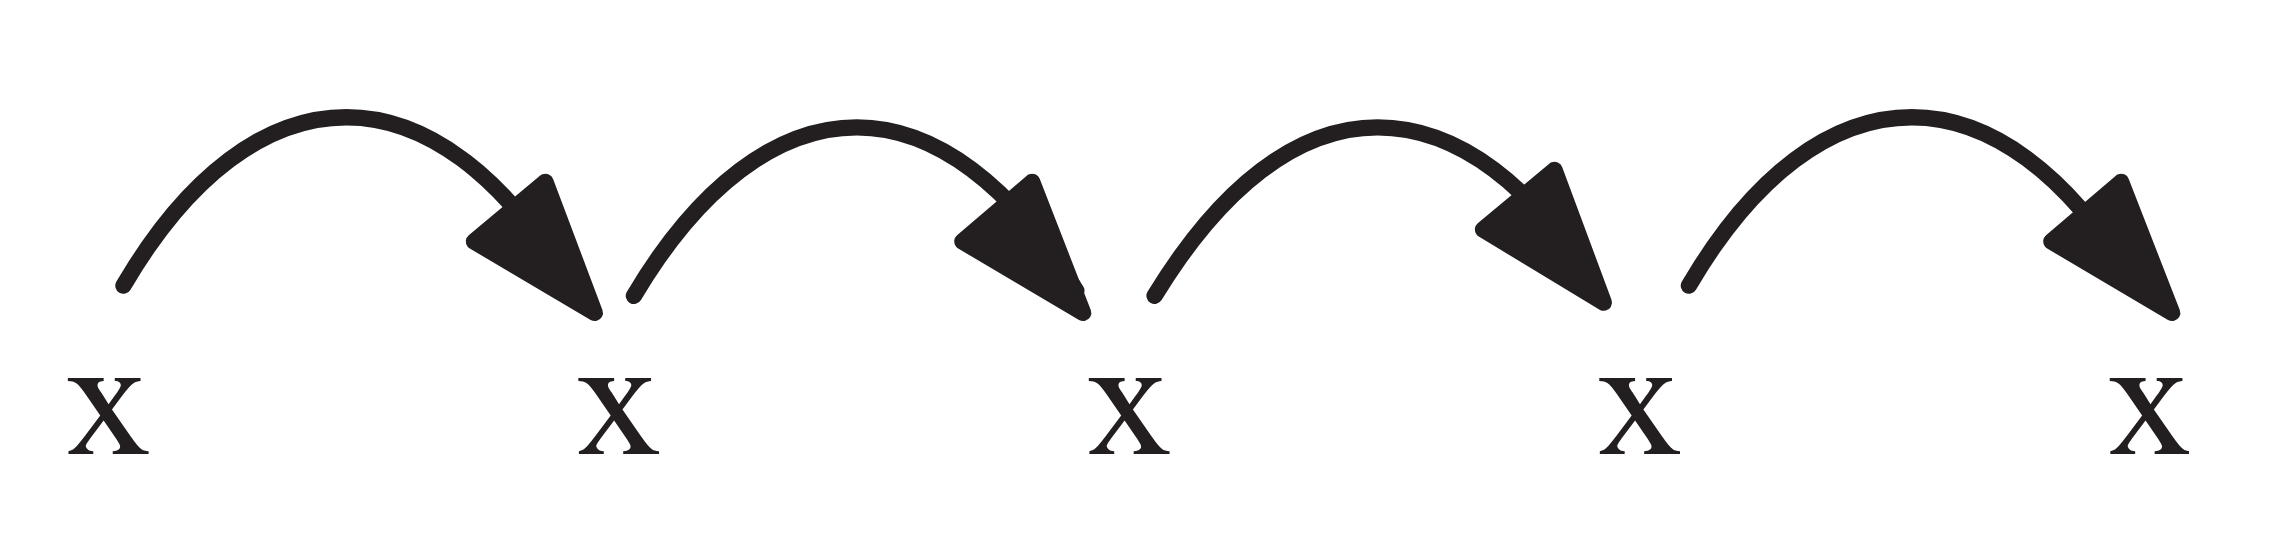
\includegraphics[width=0.3
	\textwidth] {pics/samebranching.png} \caption{Same-branching dependency direction \cite{temperley2008dependency}} 
\label{fig:samebranching} \end{figure}

\begin{figure}
	\centering 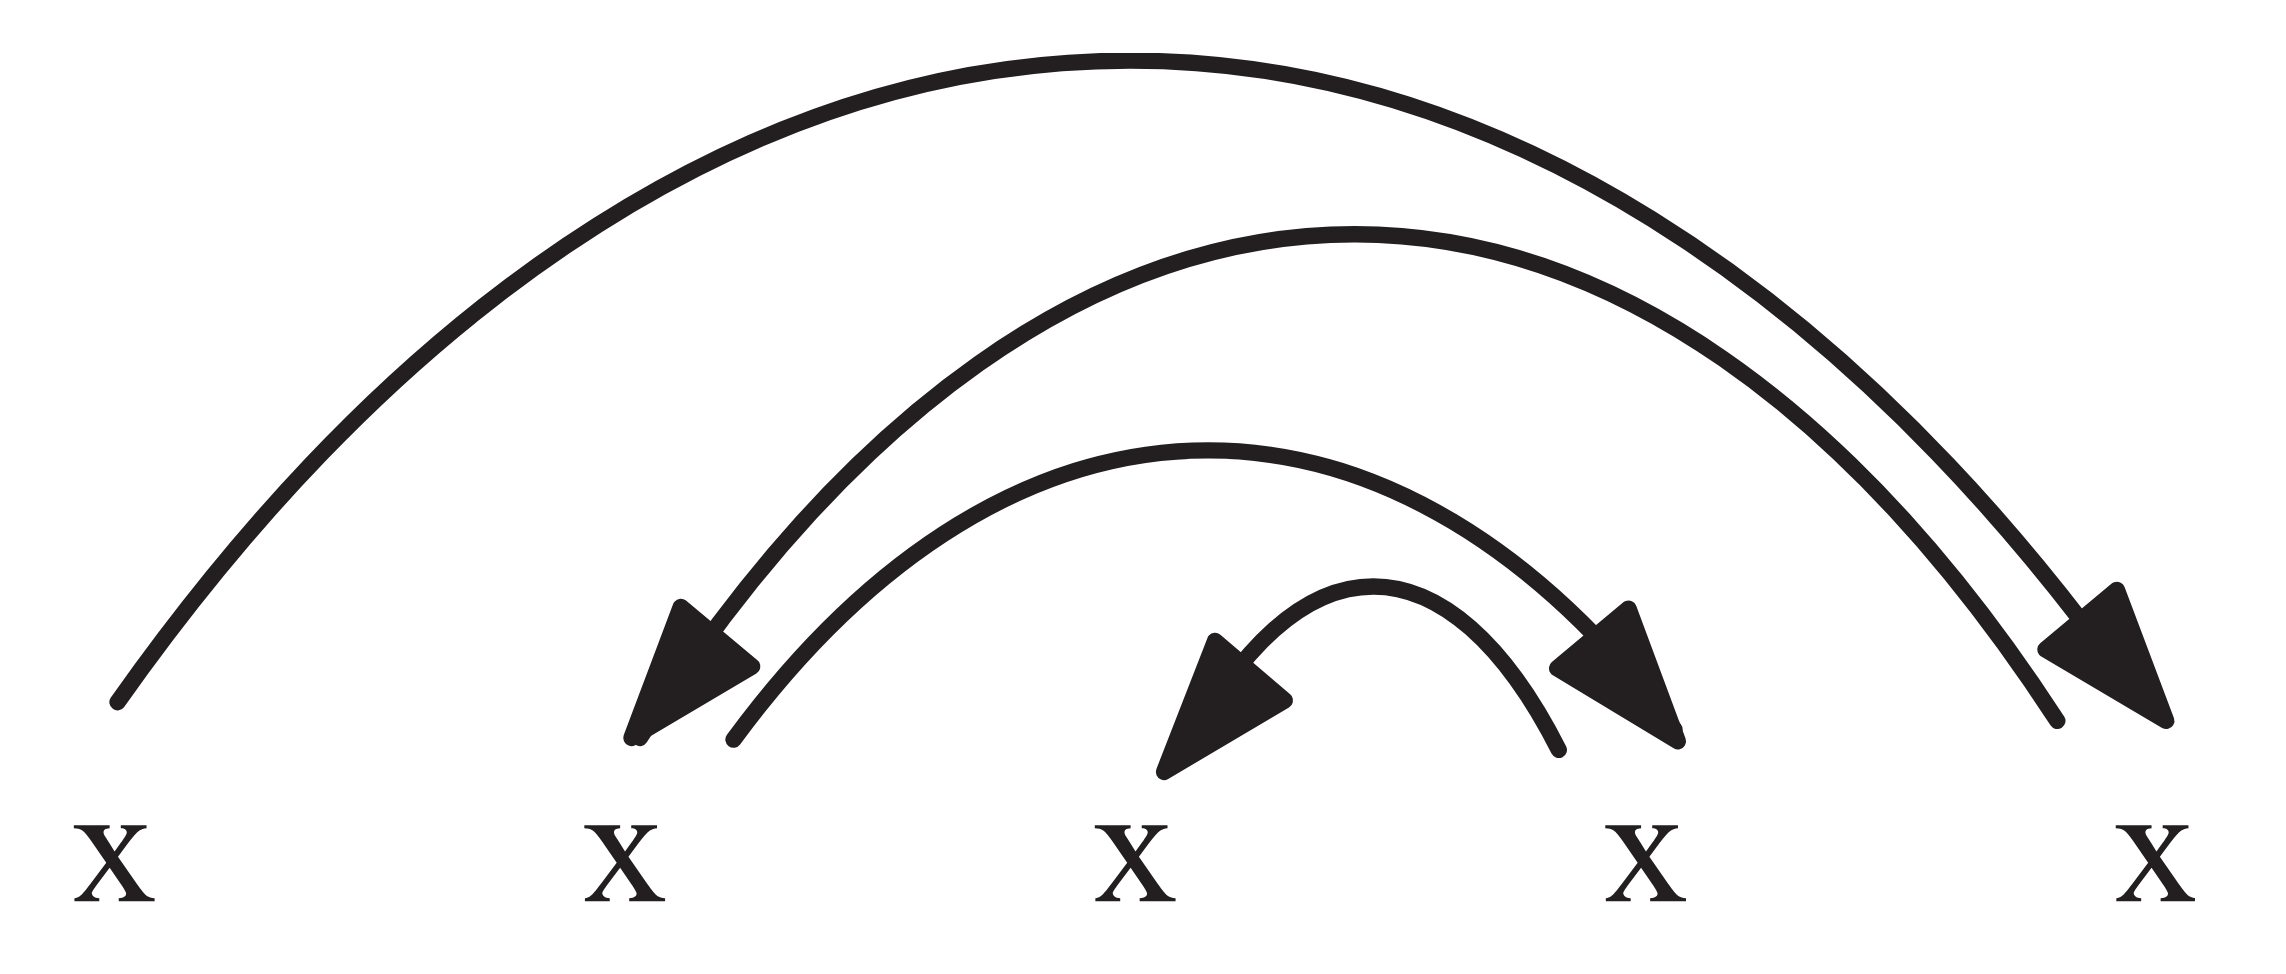
\includegraphics[width=0.3
	\textwidth] {pics/mixedbranching.png} \caption{Mixed-branching dependency direction \cite{temperley2008dependency}} 
\label{fig:mixedbranching} \end{figure}

Temperley argues that a consistent dependency direction or \textit{same-branching} is not an ideal representation of how head directionality works in real utterances \cite{temperley2008dependency}. This argument supports Dryer's research who found that the conventional view of same branching only applies on phrases consist of many constituents, while the dependency direction of phrases with single or less words are inconsistent \cite{dryer1992greenbergian}. Gildea and Temperley mentioned this research and provided empirical evidence that exhibit a combination of same branching and mixed branching (\pic~\ref{fig:mixedbranching}) dependency direction to produce a more balanced head-initial and head-final mixture to yield the shortest dependency distances (\pic~\ref{fig:balancedbranching}) \cite{gildea2010grammars}.

\begin{figure}
	\centering 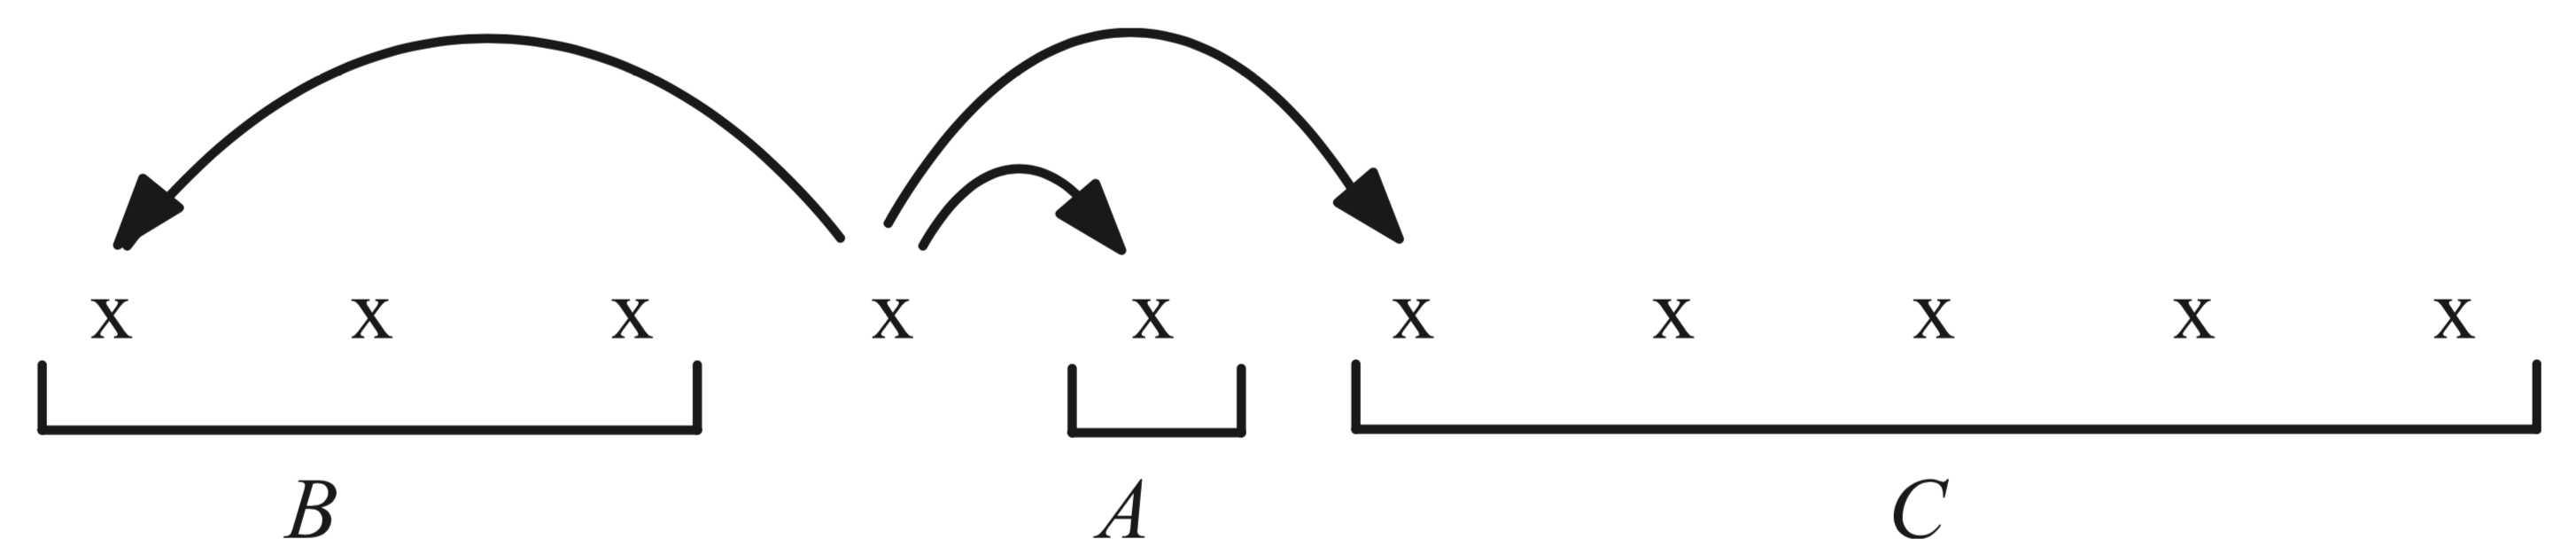
\includegraphics[width=0.45
	\textwidth] {pics/balancedbranching.png} \caption{Head-directionality balance \cite{temperley2008dependency}} 
\label{fig:balancedbranching} \end{figure}

\section{Methods}

The written data, obtained from a partnership with an Indonesian technology company called Dattabot, consists of 9311 sentences of various news articles published from 2008 to 2018. The spoken data, obtained from partnerships with various journalists across the country, consists of 10.219 sentences of live reports, interviews, and other spontaneous utterances (all in the journalistic domain) recorded from 2010 to 2018. The main challenge in including spoken data is because computational parsers are mostly trained to parse written data. Therefore, sentences with specific features of spoken language, such as hesitations, fillers, etc., are not included in the corpus. These two sets of corpora are preprocessed, parsed, and cleaned using UDPipe \cite{udpipe2017} and manual verifications. UDPipe is a trainable pipeline for tokenization, tagging, lemmatization and dependency parsing of CoNLL-U files based on dependency treebanks provided by Universal Dependencies 2.0 that are contextually adjusted for many languages, including Indonesian \cite{udpipe2017, nivre2017universal}. This study uses third party CRAN package UDPipe (version 0.5) on R programming language (version 3.3.3) \cite{udpipe2017manual, r2017project}.

The parsed data are annotated based on the parsing index to measure the dependency distances, length, and mean dependency distances. Ini the parsing index, $root$ has an index of 0. The indexing for the remaining words starts from 1. As mentioned above on Heringer's approach of measuring dependency, this study also uses the number of constituents involved in a dependency relation between two directly-linked constituents as a measuring unit. Therefore, adjacent and directly-linked constituents produce a dependency distance of 1. Data classification, subsetting, and dependency measures are performed on R and Python programming language version 3.3.3 and 3.6.3 respectively \cite{r2017project, python2017manual}. As visualized in \pic~\ref{fig:tautandependensi}, a dependency relation is illustrated through an arc with an arrow. The arrow or direction represents the hierarchy between linked constituents. For Indonesian language, an arrow pointing to the right illustrates a positive ($+$) dependency relation and denotes a head-initial dependency direction. On the other hand, an arrow pointing to the left illustrates a negative ($-$) dependency relation and denotes a head-final dependency direction.

A central node in a sentence suggests the main argument or relations of the sentence based on dependency. In a more complex sentence, a branch in a central node can contain multiple constituents. For this reason, the head directionality analysis is performed on two types of relation: (i) on directly-linked constituents in all levels of a dependency tree, including central nodes and adjacent relations, and (ii) on central nodes only, assuming all constituents under each branch are represented by the main arguments. Considering the possible influence sentence length may have on dependency distances, this study classifies both spoken and written data into five categories to acquire more accurate measures \cite{liu2017dependency, i2004euclidean, oya2011syntactic, jiang2015effects}:
\begin{itemize}
\item Sentences with 5 constituents or less.
\item Sentences with 6 to 10 constituents.
\item Sentences with 11 to 20 constituents.
\item Sentences with 21 to 30 constituents.
\item Sentences with more than 30 constituents.
\end{itemize}

\section{Results}
 
Indonesian language is considered a free-word order language \cite{sneddon2010indonesian}. However, Sneddon describes the many word order rules that put modifiers after their heads based on the functional perspective of phrase structure \cite{sneddon2010indonesian}. This study considers this functional view and uses it as a basis to see whether the tendency applies in a dependency structure. This analysis sets apart the head-first (positive) with the head-final (negative) dependency directions to capture a comprehensive characteristic based on the sentence length classifications. 

%%-----------------------------------------------------------------------------%
\subsection{Head-initial preference on all levels of a dependency structure}
%%-----------------------------------------------------------------------------%

This part of analysis measures dependency distance and number of appearance between head-initial and head-final dependency directions on all levels of a dependency structure. A full consistency of direction such as shown in \pic~\ref{fig:ts6841} and \pic~\ref{fig:ls7375} are found only in shorter sentences. \pic~\ref{fig:ts6841} illustrates a sentence with all head-initial dependency directions, in contrast to \pic~\ref{fig:ls7375}. However, the number of appearance between two speech modes is too few to be considered as a preference.

\begin{figure}
\centering
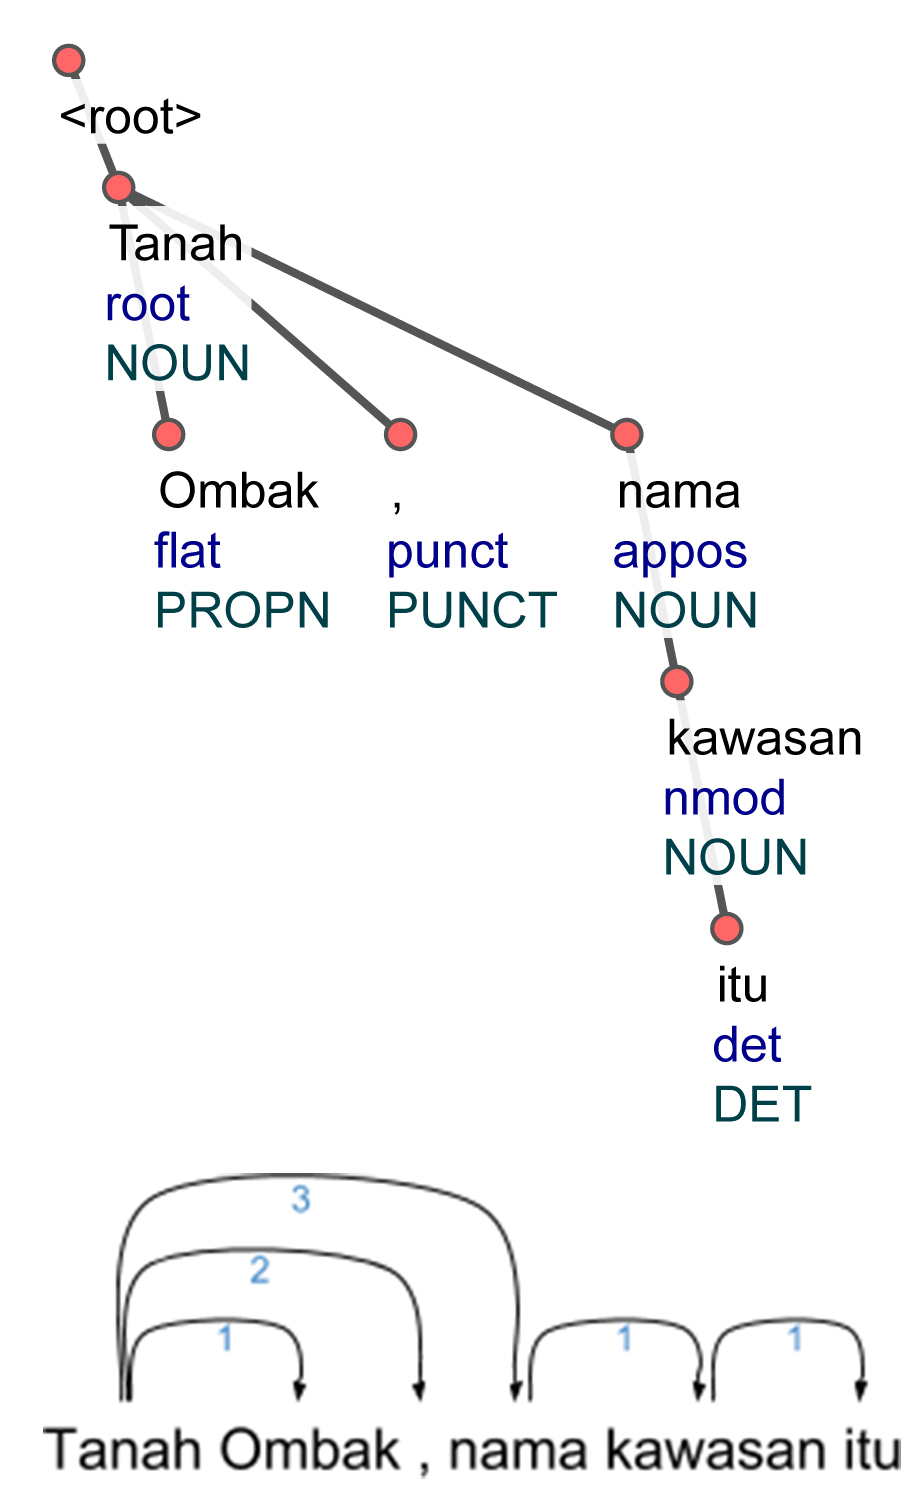
\includegraphics[width=0.45\linewidth] {pics/ts6841.jpg} 
	\caption{Sentence with all head-initial dependency directions}
	\label{fig:ts6841} 
\end{figure}

\begin{figure}
  \centering
  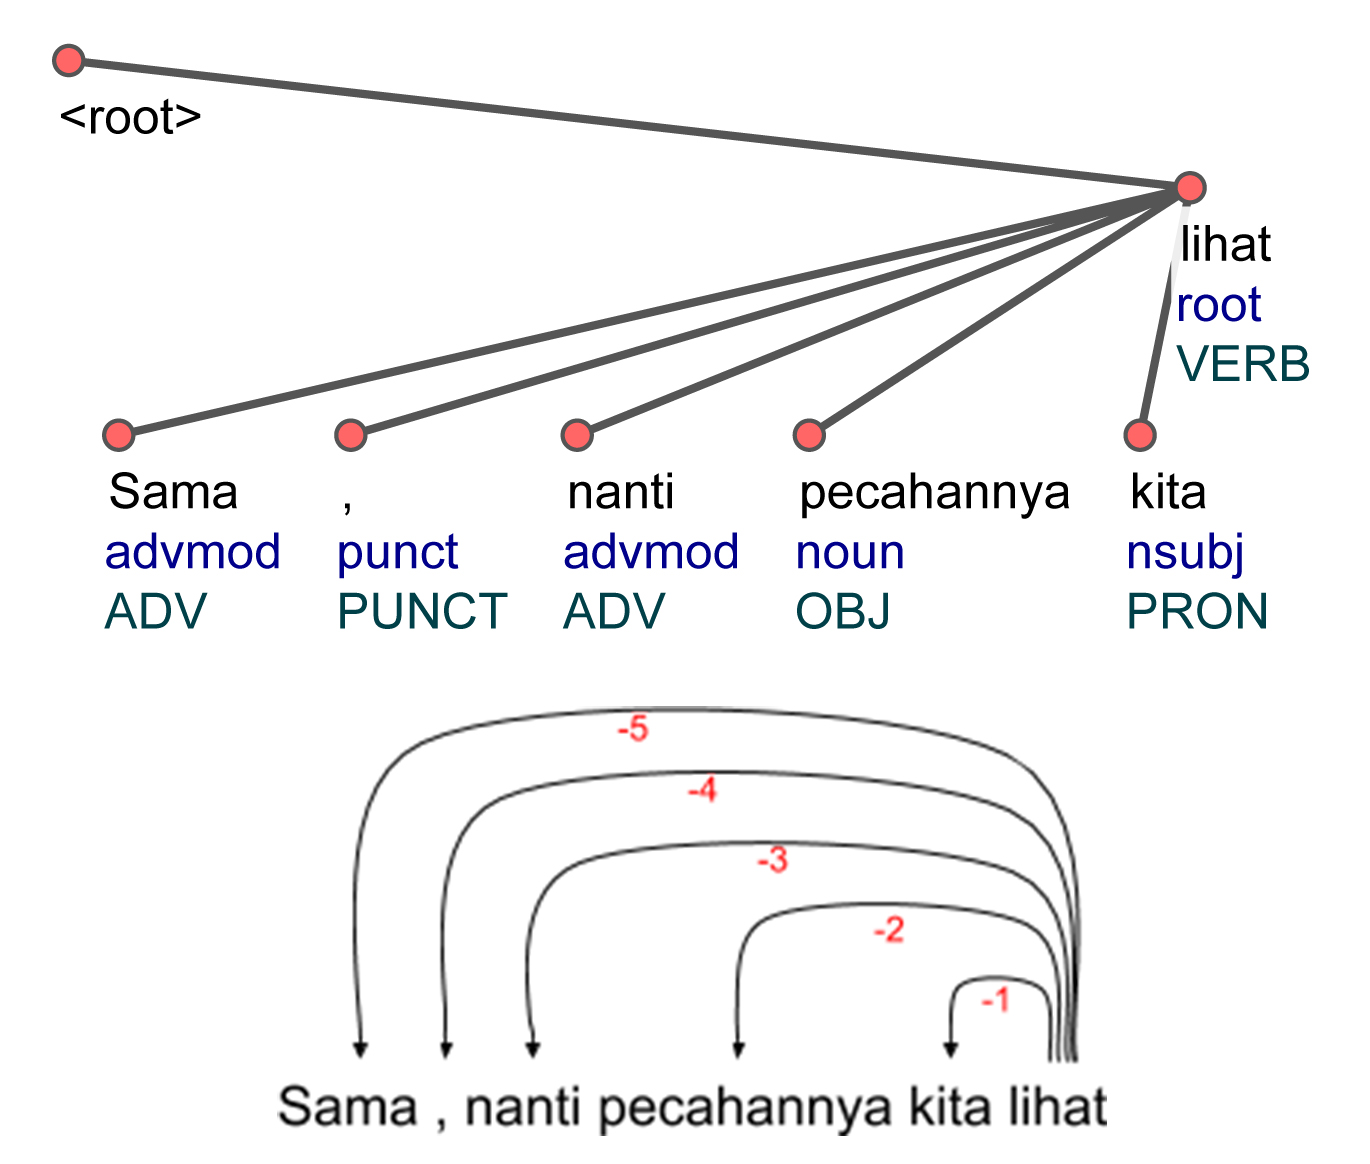
\includegraphics[width=0.7\linewidth]{pics/ls7375.jpg} 
	\caption{Sentence with all head-final dependency directions}
	\label{fig:ls7375} 
\end{figure}

As shown in \pic~\ref{fig:tulis_DLposneg} and \pic~\ref{fig:lisan_DLposneg}, both speech modes show preference towards the head-initial dependency direction. The ration difference is increasingly larger in longer sentences. There is even an indication of a threshold to reduce the distance of head-final dependency in the spoken data \pic~\ref{fig:lisan_DLposneg}. As seen in table \tab~\ref{tab:DLposneg} and \tab~\ref{tab:tautanposneg}, there are more sentences with longer head-initial dependency length and more head-initial dependencies starting from 6 constituents. The difference between both directions are increasingly larger particularly in longer sentences. However, the margins of difference are significantly larger in the written data. 

Based on descriptive statistics using both methods of dependency length (\tab~\ref{tab:deskriptif-konstituen}) and mean dependency distance (\tab~\ref{tab:deskriptif-mdd}), preference for head-initial dependencies occur mostly in adjacent relations. This finding support the application of grammar as mentioned by Sneddon who describes that many word order rules put modifiers after their heads based on the functional perspective of phrase structure \cite{sneddon2010indonesian}.  Both methods show that head-final dependencies are relatively shorter than head-first dependencies in longer sentences. While in shorter sentences, the length and distance between both directions are quite similar.


\begin{figure}
\centering
  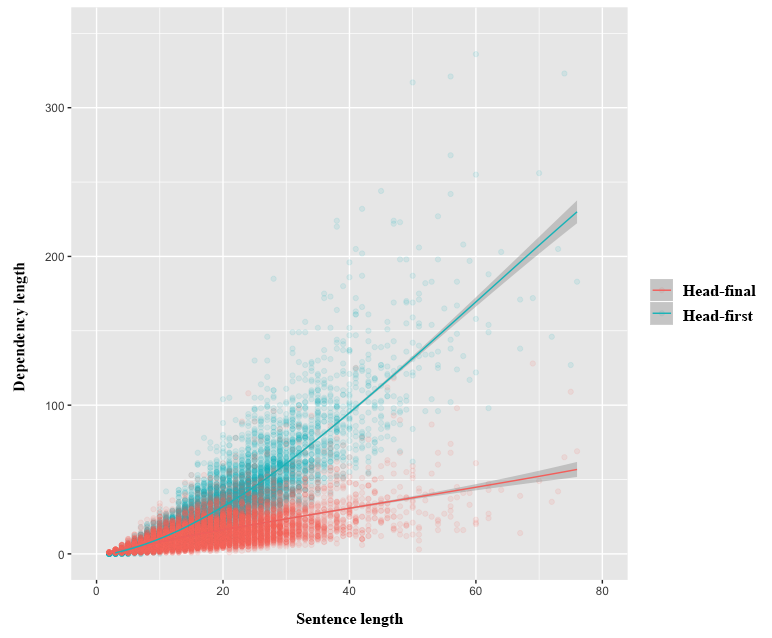
\includegraphics[width=1\linewidth] {pics/tulis_DLposneg.png} 
	\caption{Comparison of head-first and head-final dependencies on all levels based on its length in written data}
	\label{fig:tulis_DLposneg} 
\end{figure}
%
\begin{figure}
  \centering
  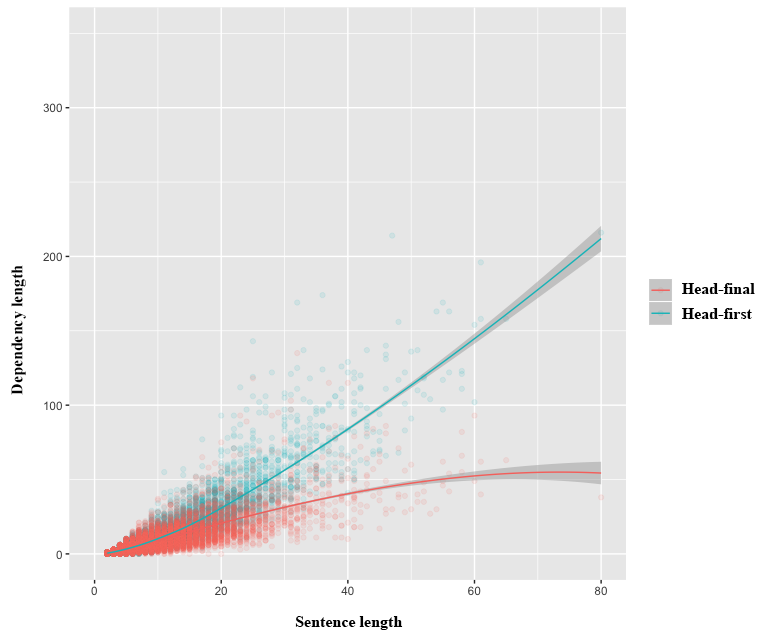
\includegraphics[width=1\linewidth]{pics/lisan_DLposneg.png} 
	\caption{Comparison of head-first and head-final dependencies on all levels based on its length in written data}
	\label{fig:lisan_DLposneg} 
\end{figure}

\begin{table}
\begin{center}
\caption{Number of occurrence where one dependency direction is more dominant than the other on all levels of a dependency structure}  \label{tab:DLposneg}
\begin{tabular}{p{1.1cm} p{1.2cm} p{1.2cm} p{1.3cm} p{1.3cm}}
\hline
Length & Written (+ \textgreater -) & Written (+ \textless -) & Spoken (+ \textgreater -) & Spoken (+ \textless -) \\ \hline
\textless= 5 & 164 & 221 & 1188 & 1354 \\
6 - 10 & 992 & 646 &1469 & 1349 \\
11 - 20 & 3145 & 952 & 1858 & 1014 \\
21 - 30 & 1854 & 200 & 644 & 166 \\
31 - 40 & 558 & 36 & 204 & 37 \\
\textgreater 40 & 201 & 5 & 89 & 7 \\ \hline
 \end{tabular}
 \end{center}
 \end{table}

\begin{table}
\begin{center}
\caption{Number of occurrence for each dependency direction on all levels of a dependency structure}  \label{tab:tautanposneg}
\begin{tabular}{p{1.1cm} p{1.2cm} p{1.2cm} p{1.3cm} p{1.3cm}}
    \hline
Length & Written (+) & Written (-) & Spoken (+) & Spoken (-) \\ \hline
\textless= 5 & 677 & 700 & 2841 & 2764 \\
6 - 10 & 7023 & 5715 & 7649 & 6918 \\
11 - 20 & 35597 & 24426 & 15554 & 12898 \\
21 - 30 & 31036 & 18163 & 7564 & 5939 \\
31 - 40 & 12904 & 6968 & 3232 & 2414 \\
\textgreater 40 & 6583 & 3240 & 1928 & 1426 \\ \hline
   \end{tabular}
\end{center}
\end{table}

\begin{table}
\begin{center}
\tiny
\caption{Jarak dependensi seluruh tautan antara dua konstituen}  \label{tab:deskriptif-konstituen}
\begin{tabular}{c l l l l l l l l l}
\hline
 & \multicolumn{4}{c}{+} & \multicolumn{4}{c}{-} & \\  \cline{2-9}  
Length & min & med	& max & mean & min & med & max & mean & \\ \cline{1-10}  
\textless= 5 	& 1 & 1 & 4 & 1,409 	& 1 & 1 & 4 & 1,606 & \multirow{6}{*}{Written}\\
6 - 10 		& 1 & 1 & 9 & 1,866 	& 1 & 1 & 9 & 1,948 & \\
11 - 20 		& 1 & 1 & 19 & 2,468 & 1 & 1 & 19 & 2,147 & \\
21 - 30 		& 1 & 1 & 29 & 2,971 & 1 & 1 & 29 & 2,241 & \\ 
31 - 40 		& 1 & 1 & 39 & 3,597 & 1 & 1 & 37 & 2,299 & \\
\textgreater 40 & 1 & 1 & 68 & 4,22 	& 1 & 1 & 55 & 2,282 & \\ 
\hline
\textless= 5 	& 1 & 1 & 4 & 1,466 	& 1 & 1 & 4 & 1,534 & \multirow{6}{*}{Spoken}\\
6 - 10 		& 1 & 1 & 9 & 1,933 	& 1 & 1 & 9 & 2,071 & \\
11 - 20 		& 1 & 2 & 19 & 2,535 & 1 & 1 & 19 & 2,321 & \\
21 - 30 		& 1 & 2 & 28 & 3,263 & 1 & 1 & 27 & 2,5 & \\ 
31 - 40 		& 1 & 2 & 37 & 3,718 & 1 & 1 & 32 & 2,657 & \\
\textgreater 40 & 1 & 2 & 66 & 4,067 	& 1 & 1 & 46 & 2,438 & \\ 
\hline
   \end{tabular}
\end{center}
\end{table}

\begin{table}
\begin{center}
\tiny
\caption{Rata-rata jarak dependensi positif dan negatif seluruh tautan antara dua konstituen}  \label{tab:deskriptif-mdd}
\begin{tabular}{c l l l l l l l l l}
\hline
 & \multicolumn{4}{c}{+} & \multicolumn{4}{c}{-} & \\  \cline{2-9}  
Length & min 	& med	& max 	& mean 	& min 	& med 	& max 	& mean 	& \\ \cline{1-10}  
\textless= 5 	& 1 		& 1 		& 3,5	 	& 1,372 	& 1 		& 1,5 	& 4	 	& 1,545 	&\multirow{6}{*}{Tulis}\\
6 - 10 		& 1 		& 1,667	& 5,2 	& 1,839 	& 1 		& 1,667 	& 9	 	& 1,895 	& 	\\
11 - 20 		& 1 		& 2,25 	& 7,25 	& 2,432 	& 1 		& 1,875 	& 10	 	& 2,117 	& 	\\
21 - 30 		& 1 		& 3,765 	& 10,278 	& 2,97 	& 1 		& 2 		& 12,75	& 2,212 	& 	\\ 
31 - 40 		& 1,458 	& 3,368 	& 9,933	& 3,595 	& 1 		& 2 		& 8		& 2,272 	& 	\\
\textgreater 40 	& 1,929 	& 3,756	& 10,567 	& 4,154 	& 1 		& 2 		& 7,111	& 2,258 	& 	\\ 
\hline
\textless= 5 	& 1 		& 1 		& 4	 	& 1,378 	& 1 		& 1,33 	& 4		& 1,456 	& \multirow{6}{*}{Lisan}\\
6 - 10 		& 1 		& 1,714	& 5,6 	& 1,867 	& 1 		& 1,8		& 9		& 2,003 	& \\
11 - 20 		& 1 		& 2,286 	& 9,625 	& 2,479 	& 1 		& 2 		& 6,818	& 2,255 	& \\
21 - 30 		& 1,4 	& 3	 	& 8,412 	& 3,252	& 1 		& 2,188	& 8,636	& 2,447 	& \\ 
31 - 40 		& 1,556 	& 3,512 	& 7,25	& 3,719 	& 1 		& 2,27	& 8,803	& 2,612 	& \\
\textgreater 40 	& 2,174 	& 3,865	& 6,895 	& 3,957 	& 1,059 	& 2,294	& 4,2		& 2,363 	& \\ 
\hline
   \end{tabular}
\end{center}
\end{table}

%%-----------------------------------------------------------------------------%
\subsection{Minimization of head-final dependency lengths and distances in longer sentences on central node level}
%%-----------------------------------------------------------------------------%
The second part of analysis measures dependency distance and number of occurrence between head-initial and head-final dependencies on central node level. \pic~\ref{fig:ls1436} and \pic~\ref{fig:ls1460} are two sentences found in the written data that have the same dependent clause \textit{kalau boleh tahu} or "if i may know" in English. Even though each sentence has a different position for this dependent clause, there is no difference in terms of their meanings. The similar example also mentioned by Sneddon in the Indonesian Reference Grammar as one of the key feature of Indonesian as a free-word order language \cite{sneddon2010indonesian}.

In \pic~\ref{fig:ls1436}, all of the constituents forming the clause \textit{kalau boleh tahu} collectively creating a head-initial dependency against its head \textit{investornya} or "the investor" in English. On the other hand, the dependent clause in \pic~\ref{fig:ls1460} creates a head-final dependency against its head \textit{ordernya} or "the order" in English. In a dependency theory, both constituents forming a dependency must be stored in the working memory until both are realized \cite{tesniere1959elements}. In this head-final dependency case, the constituents in this dependent clause (or branch of a dependency structure) must be stored as a whole until the head is realized. 

Central node level comprises of constituents that construct the main argument of a sentence. This also relates to how the root is able to bind other constituents, or its valency. To produce a more accurate overview of a main argument in a sentence, this study focuses the analysis on central node level with verbal roots. Sentences with verbal roots are found around 84,61\% or 7874 sentences in written data and 70,91\% or 7239 sentences in spoken data, which makes it the most common root type in the data.

As opposed to the analysis on all levels of a dependency structure, the preference to either dependency direction is not as clear, as seen in \pic~\ref{fig:tulisroot_DLposneg} and \pic~\ref{fig:lisanroot_DLposneg}. 


As shown in \pic~\ref{fig:tulis_DLposneg} and \pic~\ref{fig:lisan_DLposneg}, both speech modes show preference towards the head-initial dependency direction. The difference is increasingly larger in longer sentences. There is even an indication of a threshold to reduce the distance of head-final dependency in the spoken data \pic~\ref{fig:lisan_DLposneg}. As seen in table \tab~\ref{tab:DLposneg} and \tab~\ref{tab:tautanposneg}, there are more sentences with longer head-initial dependency length and more head-initial dependencies starting from 6 constituents. The difference between both directions are increasingly larger particularly in longer sentences. However, the margins of difference are significantly larger in the written data. 

Based on descriptive statistics using both methods of dependency length (\tab~\ref{tab:deskriptif-konstituen}) and mean dependency distance (\tab~\ref{tab:deskriptif-mdd}), preference for head-initial dependencies occur mostly in adjacent relations. This finding support the application of grammar as mentioned by Sneddon who describes that many word order rules put modifiers after their heads based on the functional perspective of phrase structure \cite{sneddon2010indonesian}.  Both methods show that head-final dependencies are relatively shorter than head-first dependencies in longer sentences. While in shorter sentences, the length and distance between both directions are quite similar.


\begin{figure}
  \centering
  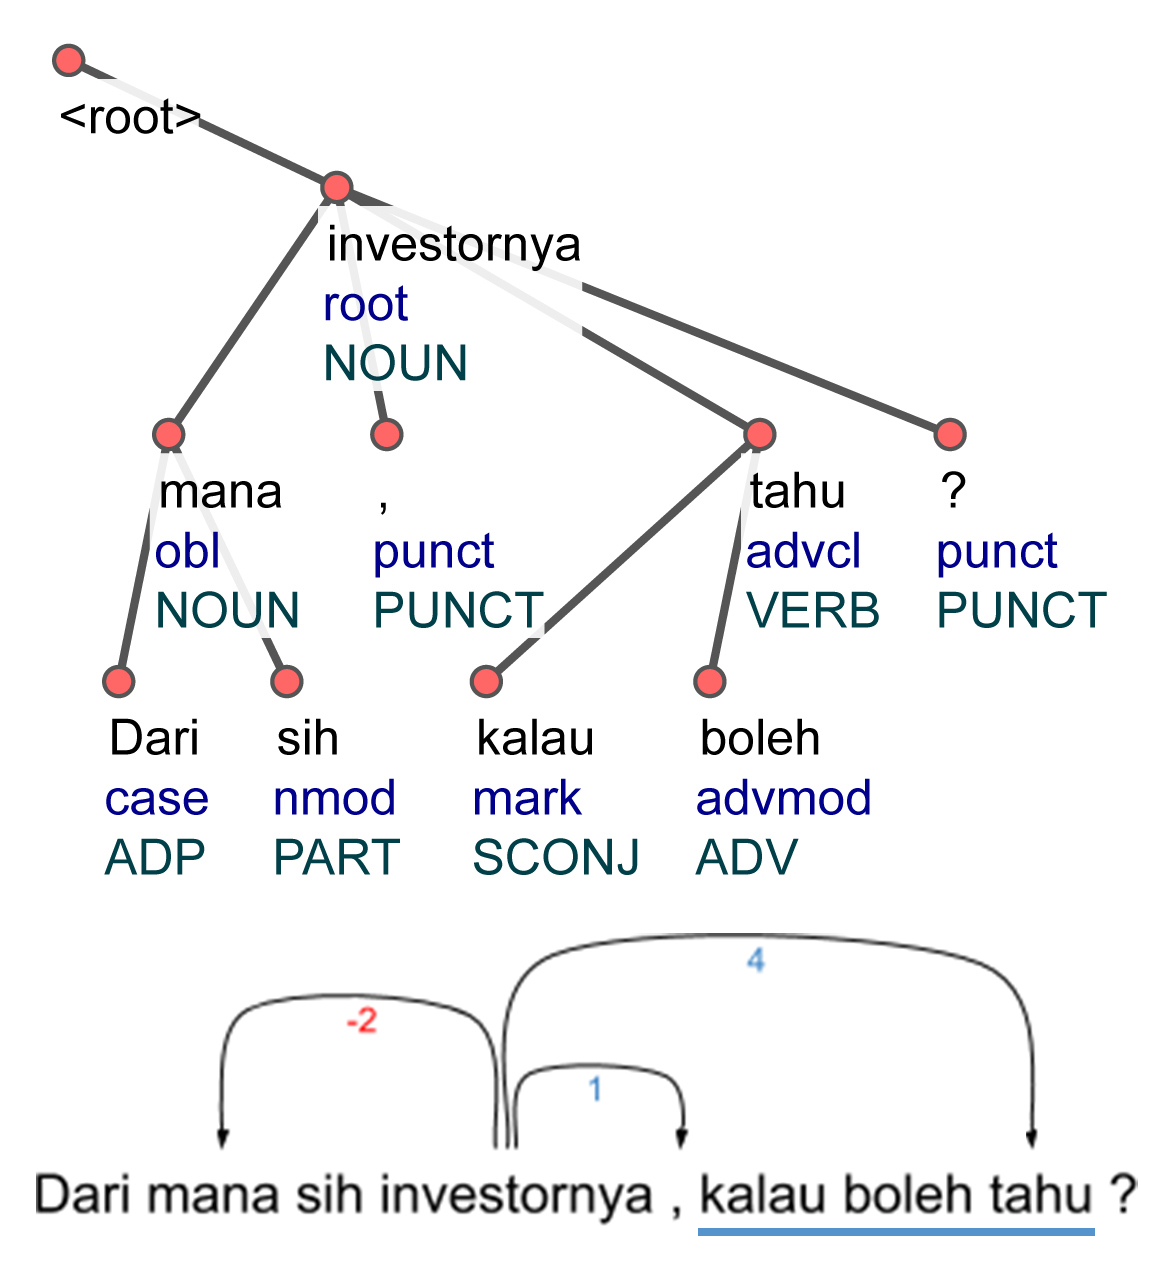
\includegraphics[width=0.55\linewidth] {pics/ls1436.jpg} 
	\caption{Sentence with a final dependent clause}
	\label{fig:ls1436} 
\end{figure}
%
\begin{figure}
  \centering
  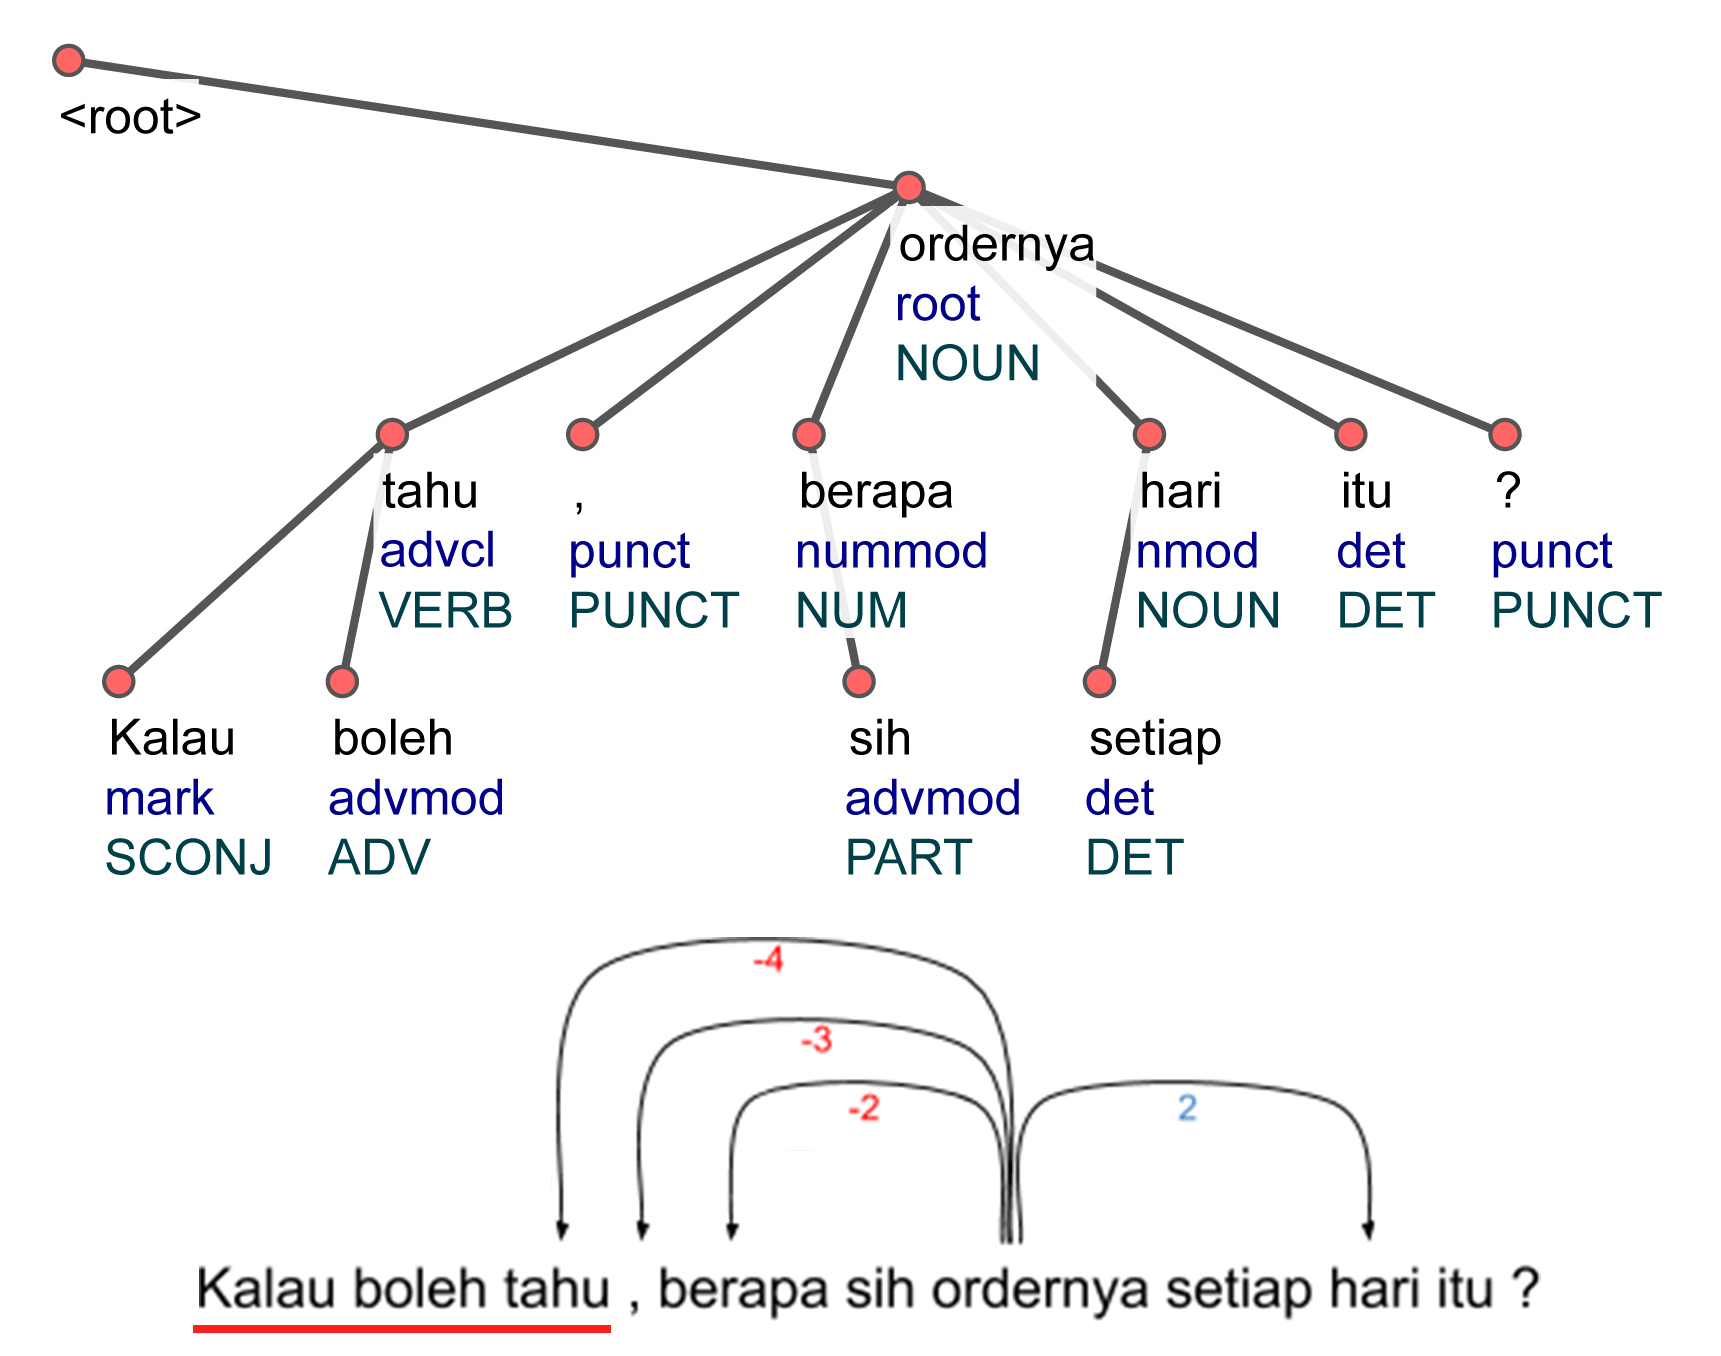
\includegraphics[width=0.75\linewidth]{pics/ls1460.jpg} 
	\caption{Sentence with an initial dependent clause}
	\label{fig:ls1460} 
\end{figure}



\begin{figure}
  \centering
  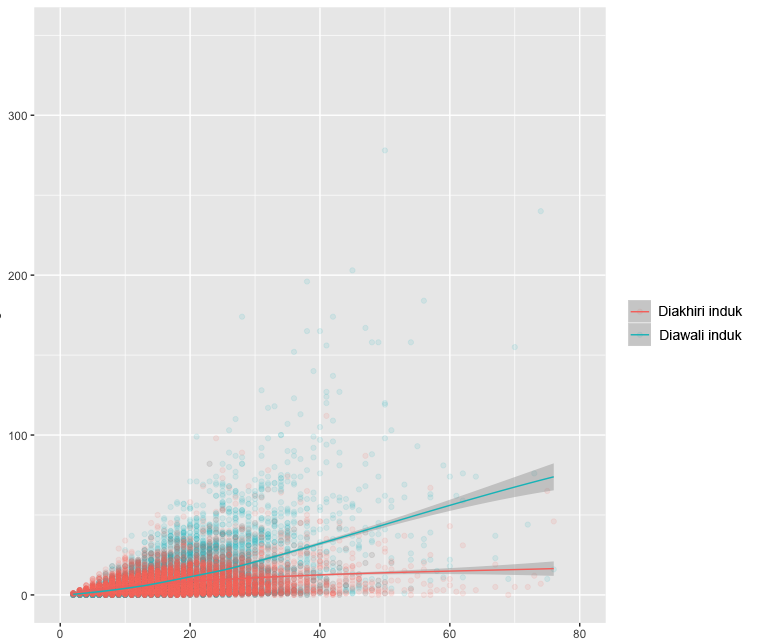
\includegraphics[width=1\linewidth] {pics/tulisroot_DLposneg.png} 
	\caption{Comparison of head-first and head-final dependencies on central node level in written data}
	\label{fig:tulisroot_DLposneg} 
\end{figure}
%
\begin{figure}
  \centering
  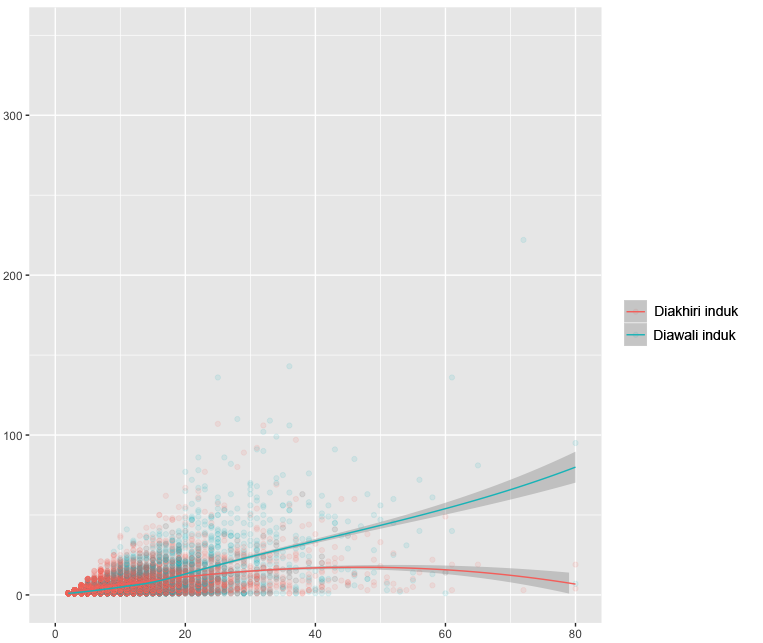
\includegraphics[width=1\linewidth]{pics/lisanroot_DLposneg.png} 
	\caption{Comparison of head-first and head-final dependencies on central node level in spoken data}
	\label{fig:lisanroot_DLposneg} 
\end{figure}

\pic~\ref{fig:tulisroot_DLposneg} dan \pic~\ref{fig:lisanroot_DLposneg} merupakan grafik panjang dependensi positif dan negatif yang didapat pada simpai pusat kalimat dengan akar berupa verba. Mayoritas frekuensi kemunculan akar verbal ini menjadi dasar untuk melihat bagaimana penutur menyusun informasi utama dengan meninjau tautan-tautan dependensi utama (simpai pusat). Oleh sebab itu, semua klausa yang mungkin terikat pada simpai cabang dianggap mengikuti induknya seperti pada contoh uraian relasi klausa \textit{kalau boleh tahu} dan akarnya di atas (\pic~\ref{fig:akarcontoh}). \pic~\ref{fig:rootDL_posneg} menunjukkan adanya konsistensi pada tingkat tautan dependensi utama dan keseluruhan kalimat. Grafik ini memperlihatkan bahwa penutur juga cenderung memilih untuk menekan penggunaan bentuk relasi diakhiri induk terutama pada kalimat panjang. Berbeda dengan \pic~\ref{fig:DL_posneg} yang pada klasifikasi kalimat menengah sudah cukup terlihat perbedaan antara panjang dependensi positif dan negatif, grafik ini menunjukkan panjang dependensi positif dan negatif saling tumpang tindih sehingga perlu ditinjau lebih dalam. Meskipun begitu, serupa dengan \pic~\ref{fig:DL_posneg}, garis regresi panjang dependensi negatif mengindikasikan adanya ambang batas pada nilai tertentu terutama pada data ragam lisan.

\begin{table}
\begin{center}
\caption{Frekuensi selisih panjang dependensi positif dan negatif pada simpai pusat akar verbal}  \label{tab:DLpusatposneg}
\begin{tabular}{p{1.1cm} p{1.2cm} p{1.2cm} p{1.3cm} p{1.3cm}}
\hline
Length & Written (+ \textgreater -) & Written (+ \textless -) & Spoken (+ \textgreater -) & Spoken (+ \textless -) \\ \hline
\textless= 5 	& 57	 	& 180 	& 393 & 1008 \\
6 - 10 		& 475 	& 796	& 655 & 1356 \\ 
11 - 20 		& 1638	& 1804	& 964 & 1336 \\
21 - 30 		& 1028	& 778	& 384 & 291 \\
31 - 40 		& 325	& 177	& 121 & 85 \\
\textgreater 40 	& 137	& 37	 	& 61 & 30 \\ \hline
   \end{tabular}
\end{center}
\end{table}

\tab~\ref{tab:DLpusatposneg} berisi jumlah-jumlah kalimat dengan melihat apakah kalimat tersebut memiliki panjang dependensi positif yang lebih jauh atau sebaliknya pada simpai pusat yang memiliki akar verbal. Berbeda dengan \tab~\ref{tab:DLposneg}, kalimat yang panjang dependensi positifnya lebih jauh ditemukan lebih banyak pada kalimat-kalimat panjang (mulai 21 konstituen). Pada ragam tulis, frekuensi keseluruhan hampir seimbang sedangkan pada ragam lisan cukup berbeda jauh (total frekuensi di mana panjang dependensi negatif lebih jauh dari panjang dependensi positif sebanyak dua kali lipat dibandingkan sebaliknya). 

\begin{table}
\begin{center}
\caption{Frekuensi tautan dependensi positif dan negatif pada simpai pusat akar verbal}  \label{tab:tautanpusatposneg}
\begin{tabular}{p{1.1cm} p{1.2cm} p{1.2cm} p{1.3cm} p{1.3cm}}
    \hline
Length & Written (+) & Written (-) & Spoken (+) & Spoken (-) \\ \hline
\textless= 5 	& 201	& 412 & 1204 & 2151 \\
6 - 10 		& 1917	& 2532 & 2998 & 4433 \\
11 - 20 		& 6914 	& 7144 & 4753 & 5570 \\
21 - 30 		& 4455	& 3691 & 1869 & 1754 \\
31 - 40 		& 1528	& 1031 & 540 & 461 \\
\textgreater 40 	& 625	& 321 & 315 & 258 \\ \hline
   \end{tabular}
\end{center}
\end{table}

\tab~\ref{tab:tautanpusatposneg} memperlihatkan bahwa pada simpai pusat akar verbal, kecenderungan menempatkan induk pada posisi sebelum konstituen terikatnya juga baru terlihat pada panjang kalimat mulai 21 konstituen. Pada kalimat-kalimat yang lebih pendek dari itu, frekuensi tautan dependensi negatif yang merepresentasikan bentuk relasi diakhiri induk justru lebih banyak. Pada data ragam tulis, total frekuensi dependensi negatif juga lebih banyak dibandingkan dependensi positif namun rasionya tidak seekstrim pada \tab~\ref{tab:DLpusatposneg}.

\begin{table}
\begin{center}
\tiny
\caption{Jarak dependensi seluruh tautan antarkonstituen pada simpai pusat akar verbal}  \label{tab:deskriptif-konstituenpusat}
\begin{tabular}{c l l l l l l l l l}
\hline
 & \multicolumn{4}{c}{+} & \multicolumn{4}{c}{-} & \\  \cline{2-9}  
Length & min 	& med	& max 	& mean 	& min 	& med 	& max 	& mean 	& \\ \cline{1-10}  
\textless= 5 	& 1 		& 1 		& 3	 	& 1,428 	& 1 		& 1		& 4	 	& 1,748 	&\multirow{6}{*}{Tulis}\\
6 - 10 		& 1 		& 2		& 9	 	& 2,336 	& 1 		& 2	 	& 9	 	& 2,571 	& 	\\
11 - 20 		& 1 		& 3	 	& 18	 	& 4,083	& 1 		& 2	 	& 19	 	& 3,61 	& 	\\
21 - 30 		& 1 		& 4	 	& 27	 	& 6,265	& 1 		& 3 		& 29		& 4,793 	& 	\\ 
31 - 40 		& 1	 	& 6	 	& 38		& 9,046 	& 1 		& 3 		& 37		& 5,925 	& 	\\
\textgreater 40 	& 1	 	& 9		& 68	 	& 12,88 	& 1 		& 3 		& 44		& 6,791 	& 	\\ 
\hline
\textless= 5 	& 1 		& 1 		& 4	 	& 1,482 	& 1 		& 1	 	& 4		& 1,69 	& \multirow{6}{*}{Lisan}\\
6 - 10 		& 1 		& 2		& 9	 	& 2,28 	& 1 		& 2		& 9		& 2,618 	& \\
11 - 20 		& 1 		& 3 		& 19	 	& 3,826 	& 1 		& 2 		& 18		& 3,658 	& \\
21 - 30 		& 1	 	& 4	 	& 26	 	& 6,413	& 1 		& 3		& 27		& 4,789 	& \\ 
31 - 40 		& 1	 	& 6	 	& 35		& 8,638 	& 1 		& 4		& 32		& 6,505 	& \\
\textgreater 40 	& 1	 	& 7		& 66	 	& 10,27 	& 1	 	& 3		& 46		& 5,852 	& \\ 
\hline
\end{tabular}
\end{center}
\end{table}

\tab~\ref{tab:deskriptif-konstituenpusat} mencakup jarak dependensi dari seluruh tautan pada simpai pusat akar verbal dan tidak dikelompokkan berdasarkan kalimatnya. Tabel ini memperlihatkan bahwa rata-rata jarak dependensi positif lebih jauh dibandingkan dependensi negatif, terutama pada kalimat yang semakin panjang. Seperti pada \tab~\ref{tab:deskriptif-konstituen}, perbandingan ini mulai terlihat pada kategori panjang kalimat 11 konstituen dan meningkat seiring bertambahnya jumlah konstituen. Pada kategori kalimat terpanjang, perbandingan jarak antara dependensi positif dan negatif juga semakin jauh. Keserupaan temuan pada simpai pusat akar verbal dan pada hubungan dua konstituen secara umum (\tab~\ref{tab:deskriptif-konstituen}) menunjukkan bahwa meskipun frekuensi dependensi negatif lebih banyak (terutama pada ragam lisan), tautan dependensi negatif ditemukan berjarak lebih pendek. Nilai tengah untuk semua ragam dan kategori panjang kalimat juga lebih mendekati ke nilai minimum, terutama pada ragam tulis. Pada kategori kalimat terpanjang ragam lisan (\textgreater 40 konstituen), rata-rata jarak dependensi negatif lebih pendek dibandingkan kategori sebelumnya (31-40 konstituen) dan perbedaan ini signifikan (\textit{P} \textless 0.05). Serupa dengan \tab~\ref{tab:deskriptif-konstituen}, mulai panjang kalimat tertentu (yang berdasarkan data ini adalah sekitar 40 konstituen), jarak dependensi negatif pada simpai pusat ragam lisan juga tidak akan melebihi nilai tertentu. 

\begin{table}
\begin{center}
\tiny
\caption{Rata-rata jarak dependensi positif dan negatif pada simpai pusat akar verbal}  \label{tab:deskriptif-mddpusat}
\begin{tabular}{c l l l l l l l l l}
\hline
 & \multicolumn{4}{c}{+} & \multicolumn{4}{c}{-} & \\  \cline{2-9}  
Length & min 	& med	& max 	& mean 	& min 	& med 	& max 	& mean 	& \\ \cline{1-10}  
\textless= 5 	& 1 		& 1 		& 3	 	& 1,363	& 1 		& 1,5		& 4	 	& 1,632	&\multirow{6}{*}{Tulis}\\
6 - 10 		& 1 		& 2		& 7	 	& 2,091	& 1 		& 2	 	& 9	 	& 2,385	& 	\\
11 - 20 		& 1 		& 3	 	& 16	 	& 3,545	& 1 		& 2,75 	& 19	 	& 3,36 	& 	\\
21 - 30 		& 1 		& 5	 	& 19,5 	& 5,514	& 1 		& 3,333	& 28		& 4,442	& 	\\ 
31 - 40 		& 1	 	& 7,5	 	& 26		& 8,044	& 1 		& 4		& 36		& 5,448	& 	\\
\textgreater 40 	& 1	 	& 11,1	& 34,286	& 11,84	& 1 		& 4,2		& 42		& 6,264	& 	\\ 
\hline
\textless= 5 	& 1 		& 1 		& 3		& 1,327	& 1 		& 1,5 	& 4		& 1,531	& \multirow{6}{*}{Lisan}\\
6 - 10 		& 1 		& 1,667	& 5,6		& 1,801	& 1 		& 2		& 9		& 2,603	& \\
11 - 20 		& 1 		& 2,286	& 7,167	& 2,479	& 1 		& 2,125	& 6,818	& 2,315	& \\
21 - 30 		& 1,4	 	& 3,118	& 8,412	& 3,375	& 1 		& 2,182	& 8,636	& 2,460	& \\ 
31 - 40 		& 1,947	& 3,643	& 7,25	& 3,879	& 1 		& 2,353	& 7,5		& 2,688	& \\
\textgreater 40 	& 2,147	 & 4,051	& 8,697	& 4,156	& 1,059	& 2,357	& 5,053	& 2,47	& \\ 
\hline
\end{tabular}
\end{center}
\end{table}

Hasil pada \tab~\ref{tab:deskriptif-mddpusat} didapatkan dengan menghitung rata-rata jarak dependensi positif dan negatif pada simpai pusat akar verbal setiap kalimat. Seperti \tab~\ref{tab:deskriptif-mdd}, distribusi nilai minimum, tengah dan maksimum pada ragam lisan juga lebih merata dibandingkan ragam tulis yang nilai tengahnya terlihat lebih mendekati nilai minimum terutama pada kalimat yang semakin panjang (mulai terlihat pada panjang kalimat 11 konstituen). Namun, perbedaannya terletak pada rata-rata jarak dependensi. Pada simpai pusat ini, rata-rata jarak dependensi ragam tulis jauh lebih besar dibandingkan ragam lisan. Seperti \tab~\ref{tab:deskriptif-konstituenpusat}, tabel ini juga memperlihatkan bahwa tautan dependensi negatif memiliki rata-rata jarak yang lebih pendek untuk kedua ragam. 

%%-----------------------------------------------------------------------------%
\subsection{Percabangan searah dan keseimbangan antara tautan dependensi positif dan negatif}
%%-----------------------------------------------------------------------------%
Pada tinjauan pustaka, pergerakan panah yang merepresentasikan direksionalitas induk dibahas menjadi dua tipe, yaitu percabangan searah (\textit{same-brancing}) dan percabangan beda arah (\textit{mixed-branching}) (\citealp{hawkins1994performance, frazier1985syntactic}). Namun, dengan jumlah konstituen yang semakin banyak dan kalimat yang semakin kompleks, direksionalitas induk tidak bisa digolongkan secara biner (hanya percabangan searah saja atau hanya percabangan beda arah saja) (\citealp{dryer1992greenbergian, temperley2008dependency}). \cite{gildea2010grammars} menjelaskan mengenai konsep keseimbangan antara tautan dependensi positif dan negatif dalam mendapatkan panjang dependensi terpendek yang juga dianalisis oleh \citep{dryer1992greenbergian}. Berdasarkan data penelitian ini, temuan yang didapatkan mendukung asumsi yang dikemukakan \cite{dryer1992greenbergian} bahwa arah dependensi tidak bisa digolongkan secara biner pada tataran kalimat, terutama pada kalimat yang semakin panjang. Namun, berdasarkan analisis dengan pemetaan kepadatan selisih antara panjang dependensi positif dan negatif, belum ditemukan kecenderungan terhadap bentuk keseimbangan tersebut. 

Pada ragam tulis, pemetaan kepadatan sangat menyebar sehingga tidak membentuk pola tertentu, sedangkan pada ragam lisan, pemetaan kepadatan terlalu memusat pada kalimat dengan jumlah konstituen sedikit sehingga juga tidak membentuk pola tertentu. Untuk mencari kecenderungan pada data seperti ini, perlu dilakukan pencarian fungsi matematis untuk menguji tingkat kesalahan (\textit{error rate}) yang lebih kecil antara kedua kemungkinan (percabangan searah atau keseimbangan dependensi positif dan negatif). Namun, pencarian fungsi matematis tersebut berada di luar batasan penelitian ini dan di luar ranah linguistik sehingga perlu dilakukan analisis lebih lanjut dari segi pembentukan model statistika. Asumsi sementara yang dapat diambil bertitik tolak dari grafik perbandingan panjang dependensi positif dan negatif pada \pic~\ref{fig:DL_posneg} dan \pic~\ref{fig:rootDL_posneg} yang dapat memberikan gambaran adanya kecenderungan untuk menghindari tautan dependensi negatif, terutama pada kalimat yang semakin panjang.

=========================================
==========================================

% An example of a floating figure using the graphicx package.
% Note that \label must occur AFTER (or within) \caption.
% For figures, \caption should occur after the \includegraphics.
% Note that IEEEtran v1.7 and later has special internal code that
% is designed to preserve the operation of \label within \caption
% even when the captionsoff option is in effect. However, because
% of issues like this, it may be the safest practice to put all your
% \label just after \caption rather than within \caption{}.
%
% Reminder: the "draftcls" or "draftclsnofoot", not "draft", class
% option should be used if it is desired that the figures are to be
% displayed while in draft mode.
%
%\begin{figure}[!t]
%\centering
%\includegraphics[width=2.5in]{tautandependensi.png}
% where an .eps filename suffix will be assumed under latex, 
% and a .pdf suffix will be assumed for pdflatex; or what has been declared
% via \DeclareGraphicsExtensions.
%\caption{Simulation Results}
%\label{fig_sim}
%\end{figure}

% Note that IEEE typically puts floats only at the top, even when this
% results in a large percentage of a column being occupied by floats.


% An example of a double column floating figure using two subfigures.
% (The subfig.sty package must be loaded for this to work.)
% The subfigure \label commands are set within each subfloat command, the
% \label for the overall figure must come after \caption.
% \hfil must be used as a separator to get equal spacing.
% The subfigure.sty package works much the same way, except \subfigure is
% used instead of \subfloat.
%
%\begin{figure*}[!t]
%\centerline{\subfloat[Case I]\includegraphics[width=2.5in]{subfigcase1}%
%\label{fig_first_case}}
%\hfil
%\subfloat[Case II]{\includegraphics[width=2.5in]{subfigcase2}%
%\label{fig_second_case}}}
%\caption{Simulation results}
%\label{fig_sim}
%\end{figure*}
%
% Note that often IEEE papers with subfigures do not employ subfigure
% captions (using the optional argument to \subfloat), but instead will
% reference/describe all of them (a), (b), etc., within the main caption.


% An example of a floating table. Note that, for IEEE style tables, the 
% \caption command should come BEFORE the table. Table text will default to
% \footnotesize as IEEE normally uses this smaller font for tables.
% The \label must come after \caption as always.
%
%\begin{table}[!t]
%% increase table row spacing, adjust to taste
%\renewcommand{\arraystretch}{1.3}
% if using array.sty, it might be a good idea to tweak the value of
% \extrarowheight as needed to properly center the text within the cells
%\caption{An Example of a Table}
%\label{table_example}
%\centering
%% Some packages, such as MDW tools, offer better commands for making tables
%% than the plain LaTeX2e tabular which is used here.
%\begin{tabular}{|c||c|}
%\hline
%One & Two\\
%\hline
%Three & Four\\
%\hline
%\end{tabular}
%\end{table}


% Note that IEEE does not put floats in the very first column - or typically
% anywhere on the first page for that matter. Also, in-text middle ("here")
% positioning is not used. Most IEEE journals/conferences use top floats
% exclusively. Note that, LaTeX2e, unlike IEEE journals/conferences, places
% footnotes above bottom floats. This can be corrected via the \fnbelowfloat
% command of the stfloats package.



\section{Conclusion}

=========================================
==========================================

Direksionalitas induk dapat menyebabkan nilai dependensi tersebut menjadi positif atau negatif. Anotasi positif menandakan bentuk relasi induk sebelum konstituen terikat (diawali induk), sedangkan anotasi negatif menandakan bentuk relasi induk setelah konstituen terikat (diakhiri induk). Berdasarkan aturan struktur frasa dalam tata bahasa yang ada (\citealp{kridalaksana2002struktur, sneddon2010indonesian}), bahasa Indonesia tergolong bahasa yang memilih bentuk relasi diawali induk dibandingkan diakhiri induk. Namun, belum ada penelitian dengan skala cukup besar yang dapat memberikan informasi ini dengan memanfaatkan data ujaran nyata karena penerapannya dalam ujaran nyata dapat bersifat tidak gramatikal namun tetap diterima. Bentuk relasi diawali induk tidak selalu menjadi preferensi pada semua bahasa karena beberapa bahasa memiliki aturan tata bahasa yang menuntut induk muncul setelah konstituen terikat atau diakhiri induk. Meskipun belum ada konvensi dan bukti empiris yang menunjukkan bahwa bentuk diawali induk lebih memudahkan proses memori kerja, \cite{futrell2015large} menunjukkan bukti empiris bahwa bahasa-bahasa yang cenderung menggunakan bentuk relasi ini memiliki tingkat pengurangan panjang dependensi lebih tinggi dibandingkan bahasa-bahasa yang cenderung menggunakan bentuk relasi diakhiri induk. 

Didukung oleh hasil penelitian ini, bahasa Indonesia menunjukkan adanya kecenderungan dalam bahasa Indonesia bahwa induk menempati posisi sebelum konstituen terikatnya} pada hubungan antara dua konstituen yang memiliki tautan langsung secara umum. Temuan ini ditandai oleh konsistensi frekuensi dan jarak dari panjang dependensi positif yang semakin besar dibandingkan panjang dependensi negatif terutama pada kalimat yang memiliki jumlah konstituen lebih banyak. Namun, pada argumen utama dengan akar verbal (yang terlihat pada simpai pusat), tidak terlihat ada kecenderungan induk menempati posisi sebelum konstituen terikatnya. Bentuk relasi diakhiri induk lebih banyak ditemukan pada kalimat dengan jumlah konstituen kurang dari 20. Sebaliknya, bentuk relasi diawali induk lebih banyak ditemukan pada kalimat yang panjang. Hal ini dapat dikaitkan dengan salah satu karakter bahasa Indonesia yang memiliki urutan kata bebas (\citealp{stack2005word, postman2004processing}). Hal ini menyebabkan dalam kondisi tertentu, urutan konstituen tersebut dapat berubah dan kalimat masih dapat diterima \citep[pp. 209-268]{sneddon2010indonesian}. 

Posisi induk terhadap konstituen terikat juga berkaitan dengan pola percabangan. Berdasarkan pemetaan dan visualisasi, kecenderungan bahasa Indonesia memanfaatkan strategi percabangan searah atau memanfaatkan strategi menyeimbangkan dependensi positif dan negatif belum terpapar dengan jelas. Penelitian lebih lanjut yang melibatkan pencarian tingkat kesalahan (\textit{margin of error}) dengan fungsi matematis perlu dilakukan untuk menjawab pertanyaan ini. Meskipun begitu, analisis kualitatif terhadap kalimat-kalimat panjang dalam ragam tulis memperlihatkan banyaknya relasi dependensi antarinduk yang bergerak menuju satu arah tertentu, sehingga menunjukkan adanya indikasi bahwa kalimat-kalimat panjang dalam bahasa Indonesia ragam tulis menerapkan strategi percabangan searah.



=========================================
==========================================

% conference papers do not normally have an appendix


% use section* for acknowledgement
\section*{Acknowledgment}


The authors would like to thank...
more thanks here \cite{zipf1949human}


% trigger a \newpage just before the given reference
% number - used to balance the columns on the last page
% adjust value as needed - may need to be readjusted if
% the document is modified later
%\IEEEtriggeratref{8}
% The "triggered" command can be changed if desired:
%\IEEEtriggercmd{\enlargethispage{-5in}}

% references section

% can use a bibliography generated by BibTeX as a .bbl file
% BibTeX documentation can be easily obtained at:
% http://www.ctan.org/tex-archive/biblio/bibtex/contrib/doc/
% The IEEEtran BibTeX style support page is at:
% http://www.michaelshell.org/tex/ieeetran/bibtex/
%\bibliographystyle{IEEEtran}
% argument is your BibTeX string definitions and bibliography database(s)
%\bibliography{IEEEabrv,../bib/paper}
%
% <OR> manually copy in the resultant .bbl file
% set second argument of \begin to the number of references
% (used to reserve space for the reference number labels box)
%\begin{thebibliography}{1}
%
%\bibitem{IEEEhowto:kopka}
%H.~Kopka and P.~W. Daly, \emph{A Guide to \LaTeX}, 3rd~ed.\hskip 1em plus
%  0.5em minus 0.4em\relax Harlow, England: Addison-Wesley, 1999.
%
%\end{thebibliography}

\bibliographystyle{IEEEtran}
\bibliography{pustaka}


% that's all folks
\end{document}


